
\documentclass[smallextended]{svjour3}[2017 April 7th]

\usepackage{amssymb}
\usepackage{amsmath,dsfont}
\usepackage[ruled,vlined, linesnumbered]{algorithm2e}
\usepackage{pgfplots}
\usepackage[utf8]{inputenc}
\usepackage{url}
\usepackage{tikz}
\usepackage{caption}
\usepackage{subfig}
\tikzset{
  font={\fontsize{9pt}{12}\selectfont}}
\newtheorem{oss}{Remark}

\newcommand{\R}{\mathbb{R}}
\newcommand{\N}{\mathbb{N}}
\DeclareMathOperator*{\argmin}{arg\,min}
\definecolor{gr}{HTML}{00BB00}
\setlength\parindent{0pt}


\begin{document}


%% Title, authors and addresses

%% use the tnoteref command within \title for footnotes;
%% use the tnotetext command for theassociated footnote;
%% use the fnref command within \author or \address for footnotes;
%% use the fntext command for theassociated footnote;
%% use the corref command within \author for corresponding author footnotes;
%% use the cortext command for theassociated footnote;
%% use the ead command for the email address,
%% and the form \ead[url] for the home page:
%% \title{Title\tnoteref{label1}}
%% \tnotetext[label1]{}
%% \author{Name\corref{cor1}\fnref{label2}}
%% \ead{email address}
%% \ead[url]{home page}
%% \fntext[label2]{}
%% \cortext[cor1]{}
%% \address{Address\fnref{label3}}
%% \fntext[label3]{}

\title{Globally convergent decomposition algorithm for risk parity problem in portfolio selection}

%% use optional labels to link authors explicitly to addresses:
%% \author[label1,label2]{}
%% \address[label1]{}
%% \address[label2]{}

\author{A.Cassioli\and G.Cocchi \and F.D'Amato\and M.Sciandrone}

\institute{A.Cassioli \at MOSEK ApS, Copenhagen, Denmark, \email{andrea.cassioli@mosek.com}}
\institute{G.Cocchi \and F.-D'Amato \and M.Sciandrone \at Dipartimento di Ingegneria dell'Informazione, Università di Firenze, Firenze, Italy, \email{guido.cocchi@unifi.it},\email{federico.damato@stud.unifi.it},\email{marco.sciandrone@unifi.it}
}

\begin{abstract}
The abstract

\end{abstract}
%% \linenumbers

%% main text
\section{Introduction}
%%write something
The most important problem in budget allocation is making a good porfolio in terms of expected return and volatility. 
A lot of models were based on the Markowitz theory, stated in 1950s, for finding portfolio in the efficient frontier. 
All these approaches are proved to be unsuitable to real contexts, due to the market unstability and the ill-conditions of the problems. 
% aggiungere diversificazione
So the scientific community did a lot of works to find a way to minimize only the risk or the diversification. 
Many naive techniques as Equally Weighting (EW) portfolios were adopted in several real contexts showing poor perfomance, altought they have good theoretical performance. 
The Risk Parity concept was proposed in \cite{qian2005} to construct a portfolio such that all the asset contributions to the total risk are equal to each other \cite{maillard}.
Many different formulations were used to deal with Risk Parity, depending also on the absence of the \emph{short-selling} constraint (i.e. $x\ge0$).
In \cite{maillard} a nonlinear nonconvex least-squares optimization model without short-selling constraint was proposed.

In \cite{tardella2016} an equally bounded risk formulation was proposed, in which all the risk contributions are equally upper bounded by the same variable. It can be proved that an optimal solution for the long-short ERB is also a Risk Parity solution with minimum variance.
In \cite{feng2016} a scalarized version of a multi-objective optimization problem considering the expected return the risk the sparsity and the risk parity was addressed with a successive convex approximations.
In \cite{tutuncu} a lightly modification of the least-squares approach was proposed considering another optimization variable $\theta$ which represents the value around which all risk contribution will stay.
\begin{subequations}\label{eq:problemRP} 
\begin{align}
\min_{x,\theta} & \quad f(x,\theta) =  \sum_{i=i}^n \left(x_i(Q x)_i - \theta\right)^2 \\
\text{s.t.} & \quad l \leq x \leq u \\
& \quad \mathds{1}^T x = 1 
\end{align}
\end{subequations}
Due to its more readable form and its lower evaluating cost, we consider that formulation as our optimization problem.
Because of Sequential Quadratic Programming has poor performance when the number of assets increases, we proposed a globally convergent decomposition algorithm which uses a two level decomposition framework.
We use a Gauss-Seidel decomposition with respect to the two blocks $x,\theta$, then when we have to optimize the $x$ block we use a Gauss-Southwell decomposition which select the Most Violating Pair for the optimality conditions among all the asset variables. Then we decrease the objective function with a line search considering only the MVP pair.

The paper proceeds as follow: in section blablablabla.


\begin{proposition}
evbrfretre
\end{proposition}
\clearpage
\section{Preliminary background}\label{sect:2}
Let us consider the following optimization problem:
\begin{subequations}\label{eq:problem} 
\begin{align}
\min_{x,y} & \quad f(x,y)  \\
\text{s.t.} & \quad l \leq x \leq u \\
& \quad \mathds{1}^T x = 1 
\end{align}
\end{subequations}
where $x \in \R^n$, $y \in \R^m$, $f$ continuously differentiable, $l, u \in \R^n$ with $l < u$ and $\mathds{1} \in \R^n$ is all composed by ones. 

We define the feasible set $\mathcal{F}$  of Problem (\ref{eq:problem}):
\begin{equation}
\mathcal{F} = \{(x,y) \in \R^{n+m} : \mathds{1}^T x = 1, l \leq x \leq u\}.
\end{equation}
A vector $d\in \R^{n+m}$ is partitioned as follows
$$
d=\left(
\begin{array}{c}
d_x\\
d_y
\end{array}
\right ),
$$
where $d_x\in R^n$ and $d_y\in R^m$.

Given $(x,y) \in \mathcal{F}$, the set of feasible directions in $(x,y)$ is the cone
\begin{equation}
 \mathcal{D}(x,y)=\{ d \in \R^{n+m}: \mathds{1}^Td_x=0, d_i\ge 0 \ \forall i \in L(x), d_i\le 0 \ \forall i \in U(x)\}
\end{equation}
where
\begin{equation}
 \begin{aligned}
  &L(x)=\{ i: \ x_i=l_i\}\\
  &U(x)=\{ i: \ x_i=u_i\}
 \end{aligned}
\end{equation}
Given $(\bar x,\bar y) \in \mathcal{F}$, we say that $(\bar x,\bar y)$ is a {\it critical point} if
$$
\nabla f(\bar x,\bar y)^Td\ge 0\quad\quad \forall d\in  \mathcal{D}(\bar x,\bar y).
$$
We can state the following result.

\begin{proposition}[Name]
\label{optimality}
A point $(\bar x,\bar y) \in \mathcal{F}$ is a critical point if and only if
\begin{equation}\label{on_x}
\begin{aligned}
&\nabla_xf(\bar x,\bar y)^Td_x\ge 0 \quad \forall d_x\in R^n & \\ 
&\text{s.t.} \quad \mathds{1}^Td_x=0,\quad d_i\ge 0 \ \forall i \in L(\bar x), \quad d_i\le 0 \ \forall i \in U(\bar x)&
\end{aligned}
\end{equation}
\begin{equation}\label{on_y}
 \nabla_yf(\bar x,\bar y)=0.
\end{equation} 
\end{proposition}


In correspondence to a feasible point $(x,y)$ we introduce the index sets
$$
R(x)=L(x)\cup C(x)
$$
$$
S(x)=U(x)\cup C(x),
$$
where 
$$
C(x)=\{i: l_i<x_i<u_i\}.
$$
We can state the following propositions (Propositions 2.2 and 2.3 in Jota2009).
\begin{proposition}\label{2.2}
 A feasible point $(\bar x,\bar y)$ is a critical point if and only if for each pair $(i,j)$,
$i\in R(\bar x)$, $j\in S(\bar x)$, we have
\begin{equation}\label{on_RS}
 {{\partial f(\bar x,\bar y)}\over{\partial x_i}}\ge
 {{\partial f(\bar x,\bar y)}\over{\partial x_j}}
\end{equation}
\begin{equation}\label{on_y2}
\nabla_yf(\bar x,\bar y)=0.
\end{equation}
\end{proposition}
\begin{proposition}\label{2.3}
 Let $\{(x^k,y^k)\}$ be a sequence of feasible points convergent to a point $(\bar x,\bar y)$.
Then, for sufficiently large values of $k$, we have
$$
R(\bar x)\subseteq R(x^k) \quad \quad {\rm and}\quad \quad S(\bar x)\subseteq S(x^k).
$$
\end{proposition}

\subsection{Set of sparse feasible directions}
In our decomposition framework we will employ feasible directions having only two
nonzero components.
Then, in this subsection we introduce these sparse feasible directions and we show their important properties.

Given $i, j\in  \{1, \ldots ,n\}$, with $i\ne j$,
we indicate by $d^{i,j}\in  \R^{n+m}$ such that
\begin{equation}\label{eq:direction}
d_h^{i,j}= 
\begin{cases}
1, \quad \text{    } h=i\\
-1, \text{    } \text{    } h=j\\
0, \quad \text{    } \text{otherwise}
\end{cases}
\end{equation}
Note that, by definition, the components $d_h^{i,j}$ with $h=n+1,\ldots,n+m$ are always set to zero.

Given $(x, y) \in \mathcal{F}$ and the corresponding index sets $R(x)$ and $S(x)$, we indicate by $D_{RS}(x,y)$
the set of directions $d^{i,j}$ with $i \in R(x)$ and $j \in S(x)$, namely
$$
D_{RS}(x,y)=\cup_{i\in R(x),j\in S(x)}d^{i,j}.
$$
\begin{proposition}\label{3.1}
Let $(\bar x,\bar y)$ be a feasible point. For each pair $i \in R(x)$ and $j \in S(x)$, the
direction $d^{i,j}\in \R^{n+m}$ is a feasible direction at $(\bar x,\bar y)$, i.e. $d \in D(\bar x,\bar y)$.
\end{proposition}
\begin{proposition}\label{3.2}
A feasible point $(\bar x,\bar y)$
 is a critical point if and only
\begin{equation}\label{on_x2}
\nabla f(\bar x,\bar y)^Td^{i,j}\ge 0\quad\quad \forall d^{i,j}\in D_{RS}(\bar x,\bar y)
\end{equation}
\begin{equation}\label{on_y3}
 \nabla_y f(\bar x,\bar y)=0.
\end{equation} 
\end{proposition}
Given a feasible point $(\bar x,\bar y)$, a pair $i\in R(\bar x)$ and $j\in S(\bar x)$ such that
$$
\nabla f(\bar x,\bar y)^Td^{i,j}<0
$$
is said a {\it Violating Pair} (VP).

A violating pair $(i^\star,j^\star)$ such that 
\begin{equation}\label{mvp}
 \nabla f(\bar x,\bar y)^Td^{i^\star,j^\star}\le \nabla f(\bar x,\bar y)^Td^{i,j} \quad \forall i\in R(\bar x), \ j\in S(\bar x).
\end{equation}
is the {\it Most Violating Pair} (MVP).



\clearpage
\section{A general decomposition framework}
The algorithm follows the Gauss-Seidel scheme with 2 blocks of variables ($x$ and $y$). At each iteration, we optimize $f$ w.r.t. one block of variables, considering the other block fixed. \\
Note that problem (\ref{eq:problem}) is not necessary convex with respect to $x$ but it is strictly convex and coercive with respect to $y$. Infact we have:
\begin{equation}
\frac{\partial^2}{d^2y} f(x,y) = 2 
\end{equation}
which is a sufficient condition for a strictly convex function. At each iteration $k$, we have 
\begin{equation}\label{eq:updatey}
y^{k+1} = \argmin_y f(x^{k},y)
\end{equation}
$f$ is strictly convex with respect to $y$, so we can find $y^{k+1}$ as a solution of
\begin{equation}
\frac{\partial f(x^{k},y)}{\partial y} = 0 
\end{equation}
That is
\begin{equation}
y^{k+1} = \frac{\sum_{i=1}^n x_i^{k} (Q x^{k})_i}{n}
\end{equation}


\begin{algorithm}[ht]
 \KwData{Given the initial feasible guess $(x^{0}, y^{0})$}
 Set $k = 0$\\
 \While{(not convergence)}{
  Compute $y^{k+1}$ as in (\ref{eq:updatey})\\
  Compute $\nabla_{x} f(x^{k},y^{k+1})$ \\
  Choose indexes $i(k), j(k)$ using the Gauss-Southwell rules \\
  Choose a step $\alpha^{k}$  along the direction $d^{i(k),j(k)}$, with QLS or ELS\\
  Set $x^{k+1} = x^{k} + \alpha^{k}d^{i(k),j(k)}$ \\
  Set $k = k + 1$
 }
 \caption{Decomposition Algorithm}
\end{algorithm}

\clearpage
%\section{Convergence analysis}
%Let us consider the following subset of indexes at $x^k$:
\begin{equation}
 \begin{aligned}
   L(x^k) =\{ i \in\{1,\ldots,n \}: x^k_i = a_i\}\\
  U(x^k) =\{i \in\{1,\ldots,n \} : x^k_i = b_i\}
 \end{aligned}
\end{equation}
Also we define set:
\begin{equation}
 C(x^k)=\{ i \in\{1,\ldots,n \}: a_i<x^k_i < b_i\}\\
\end{equation}
We use the following lemma:
\begin{lemma}\label{lem:direction}
 Let ${(x^k,y^k)} \in \mathcal{F}$ a sequence converging to $(\overline{x},\overline{y}) \in \mathcal{F}$, then for $k$ sufficiently large we have:
 
 \begin{subequations}
 \begin{align}
& \mathcal{D}(\overline{x},\overline{y}) \subseteq \mathcal{D}(x^k,y^k)\\
&L(\overline{x})\cup C(\overline{x})  \subseteq L(x^k)\cup C(x^k)\\
&U(\overline{x})\cup C(\overline{x})  \subseteq U(x^k)\cup C(x^k)
\end{align}
 \end{subequations}

\end{lemma}

\begin{proposition}
Suppose that the level set $\mathcal{L}_0$ is a compact set. Let $\{(x^k, y^k)\}$ be the sequence of points generated by the decomposition algorithm. Then
\begin{itemize}
\item $(x^k, y^k) \in \mathcal{L}_0, \enskip \forall k$ 
\item  $\{(x^k, y^k)\}$ admits limit points and each limit point is critical for Problem (\ref{eq:problem})
\end{itemize}
\end{proposition}
\begin{proof}
From (\ref{eq:updatey}) we have
\begin{equation}
f(x^{k}, y^{k+1}) \leq f(x^{k}, y^{k})
\end{equation}
and from the update rule of $x$ it follows
\begin{equation}\label{eq:dec}
f(x^{k+1}, y^{k+1}) \leq f(x^{k}, y^{k+1})
\end{equation}
Finally we have
\begin{equation}
f(x^{k+1}, y^{k+1}) \leq f(x^{k}, y^{k})
\end{equation}
so we have that the points of the sequence $\{(x^{k}, y^{k})\}$ belongs to the level set $\mathcal{L}_0$.
\vspace{1.5cm}

Let $(\overline{x},\overline{y})$ be a limit point of $\{(x^k, y^k)\}$, i.e. there exist an infinite subset $K \subseteq N$ such that
\begin{equation}\label{eq:asim}
\lim_{k \in K, k \rightarrow \infty} (x^k, y^k) = (\overline{x},\overline{y}) \qquad \lim_{k \in K, k \rightarrow \infty} d^{i(k),j(k)} = \overline{d}
\end{equation}
By contradiction, let us assume that $(\overline{x},\overline{y})$ is not a solution. In this case, at least one of the following conditions hold:
\begin{subequations}
\begin{align}
&\nabla_y f(\overline{x},\overline{y}) \neq 0  \label{eq:a}\\
&\exists \enskip i, j \enskip  \text{s.t.} \enskip \overline{x}_i > l_i \enskip  \text{and} \enskip  \nabla_x f(\overline{x},\overline{y})^T d^{i,j} = -\eta < 0 \label{eq:b}
\end{align}
\end{subequations}
For Point (\ref{eq:a}), we recall that for (\ref{eq:updatey}) $y^{k+1}$ minimizes $f(x^{k},y)$ with respect to $y$. So, if we imagine to perform QLS along a descent direction (for example, $-\nabla_y f(x^{k},y^{k})$) we have
\begin{equation}\label{eq:dis}
f(x^{k}, y^{k+1}) \leq f(x^{k}, y^{k}) - \gamma (\alpha \parallel \nabla_y f(x^{k}, y^{k}) \parallel) ^2 \qquad \forall \alpha, \gamma > 0
\end{equation}
From (\ref{eq:dis}) and thanks to (\ref{eq:dec}), we can extend the QLS convergence properties to $(x^{k+1}, y^{k+1})$. In particular, we can write
\begin{equation}
\lim_{k \in K, k \rightarrow \infty} \parallel \nabla_y f(x^{k}, y^{k}) \parallel =  \parallel \nabla_y f(\overline{x},\overline{y}) \parallel = 0
\end{equation}
So we have proved that (\ref{eq:a}) cannot hold.\\
For Point (\ref{eq:b}), the algorithm performs a QLS line search along $d^{i(k),j(k)}$ to determine the step $\alpha^{k}$. Thanks to QLS we can write
\begin{equation}\label{eq:armijoprop}
%\lim_{k \in K, k \rightarrow \infty} \alpha^{k} \parallel d^{i(k),j(k)} \parallel \frac{ \left| \nabla_x f(x^{k}, y^{k+1})^T d^{i(k),j(k)} \right|}{\parallel d^{i(k),j(k)} \parallel} = 0
\lim_{k \in K, k \rightarrow \infty} \alpha^{k} \parallel d^{i(k),j(k)} \parallel = 0
\end{equation}
From (\ref{eq:direction}), we know that $\parallel d^{i(k),j(k)} \parallel = \sqrt{2} \enskip\forall k$, so from (\ref{eq:armijoprop}) it follows
\begin{equation}\label{eq:alpha}%\label{eq:armijoprop2}
%\lim_{k \in K, k \rightarrow \infty} \alpha^{k}  \left| \nabla_x f(x^{k}, y^{k+1})^T d^{i(k),j(k)} \right| = 0
\lim_{k \in K, k \rightarrow \infty} \alpha^{k}=0
\end{equation}
From (\ref{eq:b}) and because of $\overline{d}$ is limit of steepest descent direction in $\overline{x}$  we can write
\begin{equation}\label{eq:wrong}
\lim_{k \in K, k \rightarrow \infty} \nabla_x f(x^k, y^k)^T d^{i(k),j(k)} = \nabla_x f(\overline{x},\overline{y})^T \overline{d} = \eta_1 \le \eta < 0
\end{equation}
In general, we have that
\begin{equation}
\lim_{k \in K, k \rightarrow \infty} \alpha^k \leq \lim_{k \in K, k \rightarrow \infty} \Delta^k
\end{equation}
We have to differentiate between two cases:
\begin{subequations}
\begin{align}
& \lim_{k \in K, k \rightarrow \infty} \Delta^k > 0 \label{eq:great}\\
& \lim_{k \in K, k \rightarrow \infty} \Delta^k = 0 \label{eq:zero}
\end{align}
\end{subequations}
If (\ref{eq:great}) holds, for large enough values of $k$, i.e. for $k \geq \hat{k}$, it must be $\alpha^k < \Delta^k$. From QLS properties we have at least a failure, for $k \geq \hat{k}$:
\begin{equation}\label{eq:arm1}
f(x^k + \frac{\alpha^k}{\delta} d^{i(k),j(k)}, y^k) - f(x^k,y^k) > -\gamma \left(\frac{\alpha^k}{\delta}\right)^2 ||d^{i(k),j(k)}||^2
\end{equation}
For the mean value theorem, we can write
\begin{equation}\label{eq:arm2}
f(x^k + \frac{\alpha^k}{\delta} d^{i(k),j(k)}, y^k) = f(x^k, y^k) + \frac{\alpha^k}{\delta} \nabla_x f(z^k, y^k)^T d^{i(k),j(k)}
\end{equation}
where $z^k = x^k + \vartheta_k \frac{\alpha^k}{\delta} d^{i(k),j(k)}$ and $\vartheta_k \in (0,1)$. From (\ref{eq:arm2}) and (\ref{eq:arm1}), for $k \geq \hat{k}$, we have
\begin{equation}\label{eq:nabla}
\nabla_x f(z^k, y^k)^T d^{i(k),j(k)}  >- \gamma \frac{\alpha^k}{\delta} ||d^{i(k),j(k)}||^2
\end{equation}
Using (\ref{eq:asim}) and (\ref{eq:alpha}) it must be
\begin{equation}
\lim_{k \in K, k \rightarrow \infty} z^k = \lim_{k \in K, k \rightarrow \infty} x^k + \vartheta_k \frac{\alpha^k}{\delta} d^{i(k),j(k)} = \overline{x}
\end{equation}
Taking the limit value of each member of (\ref{eq:nabla}) we have
\begin{equation}
\nabla_x f(\overline{x},\overline{y})^T \overline{d} \geq 0 %\gamma \nabla_x f(\overline{x},\overline{y})^T \overline{d}
\end{equation}
which contradicts that $\exists i,j$ such that $\overline{x}_i >l_i$ and:
\begin{equation}
\nabla_x f(\overline{x},\overline{y})^T d^{i,j} =\eta <0
\end{equation}

%that does not hold, since $\gamma < 1$. So we have proved that, if (\ref{eq:great}) holds, (\ref{eq:b}) cannot hold. \\

%If (\ref{eq:zero}) holds, we have to define the following subset of indexes, for all iteration $k$:

In next iterations $k+m$, $m\ge 0$ we have at least one of these two possible cases, from MVP selection rule:
\begin{subequations}
\begin{align}
 j(k+m) &\in L(x^{k+m+1})\label{eq:SetCasesA}\\
 i(k+m) &\in U(x^{k+m+1})\label{eq:SetCasesB}
\end{align}
\end{subequations}

Now we define two sets $\Gamma_1,\Gamma_2$ such that the first one contains all indexes $m \in\{0,\ldots,2n\}$ such that \ref{eq:SetCasesA} hold.
On the contrary the second one contains all indexes $m \in\{0,\ldots,2n\}$ such that \ref{eq:SetCasesB} hold.

Because of $|\Gamma_1|+|\Gamma_2|\ge2n+1$, one of these set have more than $n$ elements. Without loss of generality we take $|\Gamma_1|> n$.

Then there exist at least two indexes $0\le h(k)< m(k)\le 2n$ such that:
\begin{equation}
 i(h(k))=i(m(k))=i^*
\end{equation}

We can define a subset $K \subseteq \{0,1,\ldots\}$ such that $\forall k_i \in K$ holds:
\begin{equation}
 i(k_i)=i^*
\end{equation}
and:
\begin{equation}
 k_i <k_{i+1} \le k_i+2n
\end{equation}

For the MVP selection rule $\forall k_i \in K$ must hold:
\begin{equation}
 \frac{\partial f(x^{k_i},y^{k_i})}{dx_{i^*}} \le \frac{\partial f(x^{k_i},y^{k_i})}{dx_{h}}, \ \forall h \in L(x^{k_i}) \cup C(x^{k_i})
\end{equation}

But  $\forall k_i \in K,\exists p(k_i)$ with  $k_i <p(k_i)<k_{i+1}$ such that:
\begin{equation}
 i^* \not \in U(x^{p(k_i)+1})
\end{equation}
and then
\begin{equation}
 \frac{\partial f(x^{p(k_i)},y^{p(k_i)})}{dx_{i^*}} \ge \frac{\partial f(x^{p(k_i)},y^{p(k_i)})}{dx_{h}}, \ \forall h \in U(x^{p(k_i)}) \cup C(x^{p(k_i)})
\end{equation}


Thanks to Lemma (\ref{lem:direction}) we can say that for $k$ sufficiently large, the set of feasible direction in $(x^k,y^k)$ contains the correspondent set in $(\overline{x},\overline{y})$.

Then for $k_i \in K_1 \subset K$, $k_i$ sufficiently large, then following \ref{eq:b} we have:
\begin{equation}
\begin{aligned}
i \in L(x^{k_i},y^{k_i}) \cup C(x^{k_i},y^{k_i})\\
j \in U(x^{k_i},y^{k_i}) \cup C(x^{k_i},y^{k_i})\\
\end{aligned}
\end{equation}
and:
\begin{equation}\label{eq:direction1}
\begin{aligned}
 \frac{\partial f(x^{k_i},y^{k_i})}{dx_{i^*}} &\le \frac{\partial f(x^{k_i},y^{k_i})}{dx_{i}}\\
 \frac{\partial f(x^{p(k_i)},y^{p(k_i)})}{dx_{i^*}} &\ge \frac{\partial f(x^{p(k_i)},y^{p(k_i)})}{dx_{j}}
 \end{aligned}
\end{equation}

Because of  definition of $K_1$ we can say that:
\begin{equation}
 \lim_{k_i \in K_1, k_i \rightarrow \infty} x^{k_i} =\overline{x}
\end{equation}
Quadratic line search guarantees that:
\begin{equation}
 ||x^{k+2n}-x^{k}|| \rightarrow 0
\end{equation}


Hence because of $p(k_i)-k_i \le 2n$ we have:
\begin{equation}
 \lim_{k_i \in K_1,k_i\rightarrow \infty}  ||x^{p(k_i)}-x^{k_i}||=0
\end{equation}
Then:
\begin{equation}
 \lim_{k_i \in K_1,k_i\rightarrow \infty} x^{p(k_i)}=\overline{x}
\end{equation}

At limit point $\overline{x}$, from equation (\ref{eq:direction1})  we have: 
\begin{equation*}
 \frac{\partial f(\overline{x},\overline{y})}{dx_i} - \frac{\partial f(\overline{x},\overline{y})}{dx_{j}} \ge 0
\end{equation*}




which contradicts \ref{eq:b}.

\end{proof}
%\clearpage
\section{An use case: Risk Parity portofolios}
In this section, we show that the general framework presented above can be used to a specific class of portfolio selection problem, namely the Risk Parity portfolio selection. We use volatility as risk measure of the fully invested portfolio, i.e.
\begin{equation}
\mathcal{R}(x) = \sigma(x) = \sqrt{x^T Q x}
\end{equation}
where $Q$ is the covariance matrix. Using the Euler decomposition, we can express the total risk as the sum of contributions from each asset in the portfolio:
\begin{equation}
\mathcal{R}(x) = \sum_{i=1}^n RC_i 
\end{equation}
where $RC_i$ is the risk contribution of the $i$-th asset, that has the form
\begin{equation}
RC_i = x_i \frac{\partial \mathcal{R}(x)}{\partial x_i}
\end{equation}
In the Risk Parity formulation, our aim is to satisfy the following set of constraints:
\begin{equation}\label{eq:rpconst}
x_i \frac{\partial \mathcal{R}(x)}{\partial x_i}= x_j \frac{\partial \mathcal{R}(x)}{\partial x_j} \quad \forall i,j
\end{equation}
We can also express (\ref{eq:rpconst}) in the following equivalent way:
\begin{equation}
x_i (Q x)_i = x_j (Q x)_j \quad \forall i,j
\end{equation}
In \cite{maillard} is proposed a least-square approach for solving the Risk Parity problem:
\begin{subequations}
\begin{align}
\min_x & \quad \sum_{i=i}^n \sum_{j=1}^{n}\left(x_i(Q x)_i - x_j(Q x)_j\right)^2\\
\text{s.t.} & \quad l \leq x \leq u \\
& \quad \mathds{1}^T x = 1 
\end{align}
\end{subequations}
The formulation proposed in \cite{tutuncu} introduces a free variable $\theta$ that is also optimized:
\begin{subequations}\label{eq:problemRP} 
\begin{align}
\min_{x,\theta} & \quad f(x,\theta) =  \sum_{i=i}^n \left(x_i(Q x)_i - \theta\right)^2 \\
\text{s.t.} & \quad l \leq x \leq u \\
& \quad \mathds{1}^T x = 1 
\end{align}
\end{subequations}
where $x \in \R^n$, $\theta \in \R$, $f$ continuously differentiable, $l, u \in \R^n$ with $l < u$ and $\mathds{1} \in \R^n$ is all composed by ones. \\
It is easy to see that Problem (\ref{eq:problemRP}) is a specific case of Problem (\ref{eq:problem}). Note that the formulation (\ref{eq:problemRP}) is non-convex, but $f(x,\theta)$ is quadratic and strictly convex with respect to $\theta$.  If the optimization problem above has an optimal value of zero, then the RP portfolio is achieved. Otherwise, the value of $\sum_{i=i}^n \left( x_i(Q x)_i - \theta\right)^2$  can be regarded as a minimum variance measure towards our goal. Note that, since (\ref{eq:problemRP}) is a non-convex problem, in theory it is hard to solve and may produce local solutions. Anyway, we have the following lemma (for the proof see \cite{tutuncu}):
\begin{lemma}\label{rplemma}
Let $f(x,\theta) = \sum_{i=i}^n \left( x_i(Q x)_i - \theta\right)^2$. A solution pair $\{x,\theta\}$ is a global optimum with $f(x,\theta)=0$ if and only if $\nabla_xf(x,\theta) = 0$ and $\frac{\partial f(x,\theta)}{\partial \theta} = 0$.
\end{lemma}
Lemma (\ref{rplemma}) implies that if constraints of (\ref{eq:problemRP}) are not considered, then the first order optimality conditions determine the global optimal solution. On the other hand, when constraints are imposed, local optima and local stationary points can occur.
\subsection{Proximal Point modification}
In this subsection we propose a \emph{Risk-Parity} version of general decomposition algorithm described above, using proximal point approximation.

Let us redefine selected variable $x_{i(k)},x_{j(k)}$ as $x_{i},x_{j}$ for ease of notation, and let us consider the step when $\theta$ is fixed (i.e $f(x,\theta)=f(x)$).

The idea behind proximal point modification is that at every iteration $k$, fixed other variable $\theta$, it's easy to solve the subproblem:
\begin{align}
 &\min_{x_i,x_j}h(x_i,x_j)= f(x_i,x_j)+ \frac{1}{2} \tau||(x_i,x_j)-(x_i^k,x_j^k)||^2\\
 &x_i+x_j = \underbrace{1-\sum_{h \ne i,j} x^k_h}_{c^k}\\
 &l \le x_i,x_j\le u
 \end{align}
where $f$ is defined in \ref{eq:problemRP} and $\tau>0$.

In fact, due to simplex constraint, the objective function depends only on one of the selected variables (e.g. $x_j$) and $f$ become 4-degree polynomial in $x_j$.

Because of $h$ is continuously differentiable, it admits minimum in a compact set and we have to search it between zeros of $h'(\xi)$ and the limit points of the feasible set.

Hence, at every iteration $k$, we can define the set of possible global minima as:
\begin{equation}
 O_k = \{ \xi < x_j^k: h'(\xi)=0\} \cup \{\min\{l_j,x_i^k\} \}
\end{equation}

then we set:
\begin{equation}
x_j^{k+1}= \arg \min_{\xi \in O_k} \{h(\xi)\}
\end{equation}
and:
\begin{equation}
x_i^{k+1}= c^{k}-x^{k+1}_j
\end{equation}



\begin{algorithm}[ht]
 \KwData{Given the initial feasible point $(x^{0}, \theta^{0})$}
 Set $k = 0$\\
 \While{(not convergence)}{
   Compute $\theta^{k+1}$ such that $f(x^{k},\theta^{k+1})\le f(x^{k},\theta^k)$ and $\nabla_\theta f(x^{k},\theta^{k+1})=0$\\
 \eIf{$k \enskip \text{mod} \enskip M = 0$}
  {
  Let $(i(k), j(k))$ be a Most Violating Pair\\ 
  }
  {
  Let $(i(k), j(k))$ be a Violating Pair\\ 
  }
  Compute $\displaystyle x_{i(k)},x_{j(k)}\in \arg \min_{\xi,\zeta} f(\xi,\zeta)+\frac{1}{2}\tau ||(\xi,\zeta)-(x_{i(k)}^k,x_{j(k)}^k)||^2$\\
  Set $k = k + 1$
 }
 \caption{Decomposition Algorithm with proximal point}
\end{algorithm}
We can prove the follwing global convergence results.
\begin{proposition}
Suppose that the level set $\mathcal{L}_0$ is a compact set. Let $\{(x^k, \theta^k)\}$ be the sequence of points generated by the decomposition algorithm with proximal point modification. Then
\begin{itemize}
\item $(x^k, \theta^k) \in \mathcal{L}_0, \enskip \forall k$ 
\item  $\{(x^k, \theta^k)\}$ admits limit points and each limit point is critical for Problem (\ref{eq:problemRP})
\end{itemize}
\end{proposition}
\begin{proof}
The firts assertion is given by algorithm statement which say:
\begin{equation}
f(x^{k+1},\theta^{k+1})\le f(x^{k+1},y^k)\le f(x^k,\theta^k)- \underbrace{\frac{1}{2}\tau ||x^{k+1}-x^{k}||^2}_{>0}
\end{equation}
then the sequence $\{(x^k,\theta^k)\} \in \mathcal{L}_0$.

To prove the second assertion it is necessary to show that
\begin{equation}
\lim_{k \rightarrow \infty} ||(x^{k+1},\theta^{k+1})-(x^{k},y^{k})||=0
\end{equation}
then the convergence can be completed as in previous proposition.

Let us start to prove that $||x^{k+1}-x^{k}||\to0$.

From the $\mathcal{L}_0$ compactness we can say that the sequence $\{(x^k,\theta^k)\}$ has a subsequence $K \subset \{0,1,\ldots\}$ convergent to $(\overline{x},\overline{y}) \in \mathcal{L}_0$. Then for the continuity of $f$ we have:
\begin{equation}
\lim_{k \in K, k \rightarrow \infty}f(x^k,\theta^k)=f(\overline{x},\overline{\theta})= \overline{f}
\end{equation}

The instruction of algorithm imply that:
\begin{equation}
f(x^{k+1},\theta^{k+1})\le f(x^{k+1},\theta^{k})\le f(x^k,\theta^k)
\end{equation}
then the sequence $f(x^k,\theta^k)$ is decreasing and lower-bounded by $\overline{f}$ then we have:
\begin{equation}
\lim_{k \in K, k \rightarrow \infty} f(x^{k+1},\theta^{k})-f(x^{k},\theta^{k})=0
\end{equation}

Proximal point step imply that:
\begin{equation}
f(x^{k+1},y^{k})+\frac{1}{2}\tau||x^{k+1}-x^{k}||^2 \le f(x^{k},y^{k})
\end{equation}

Taking the limit for $k \in K, k \to \infty$ we obtain:
\begin{equation}
\lim_{k \in K,k \to \infty} ||x^{k+1}-x^{k}||=0
\end{equation}

Now we have to prove that $|\theta^{k+1}-\theta^{k}|\to 0$, using the property that $f$ is quadratic and strictly convex with respect to $\theta$. 
We have to prove the following lemma:
\begin{lemma}
Let $f(x, \theta)$ defined in (\ref{eq:problemRP}). Then, if $\enskip\lim_{k \to \infty} f(x^{k},\theta^k)-f(x^{k},\theta^{k+1})=0$ then:
\begin{equation}
 \lim_{k\to \infty} |\theta^{k+1} -\theta^k| = 0 
\end{equation}
\end{lemma}

\begin{proof}
The instructions of the algorithm imply that at every iteration $k$, we have to select the optimal step $\alpha_k^*$ along $-\nabla_{\theta}f(x^{k},\theta^{k})$.

Because of $f$ is strictly convex quadratic function with respect to $\theta$ we have:
\begin{equation}\label{eq:quadratic}
f(x^{k},\theta^k-\alpha^*_k\nabla_{\theta}f(x^{k},\theta^{k})) = f(x^{k},\theta^{k})-\alpha^*_k |\nabla_{\theta}f(x^{k},\theta^{k})|^2
\end{equation}
with:
\begin{equation}\label{eq:upTheta}
 \theta^{k+1}= \theta^{k}-\alpha^*_k\nabla_{\theta}f(x^{k},\theta^{k})
\end{equation}

From hypothesis we have that:
\begin{equation}
 \lim_{k \to \infty} f(x^{k+1},\theta^k)-f(x^{k+1},\theta^{k+1})=0
 \end{equation}

and from \ref{eq:upTheta} and \ref{eq:quadratic} :
\begin{equation}
  \lim_{k\to \infty} |\theta^{k+1} -\theta^k| = 0 
\end{equation}
\end{proof}
 
Next convergence steps are the same used in the proof of Proposition \ref{prop:conv1}.
\end{proof}

\begin{oss}
In computational experiments we use $\tau = 0$ and compute an exact line search along direction $d^{i(k),j(k)}$. In next section we will show that in practical cases exact line search performs very well especially increasing number of variables.
\end{oss}



\clearpage
\section{Computational experiments}

\begin{figure}
\makebox[\textwidth][c]{
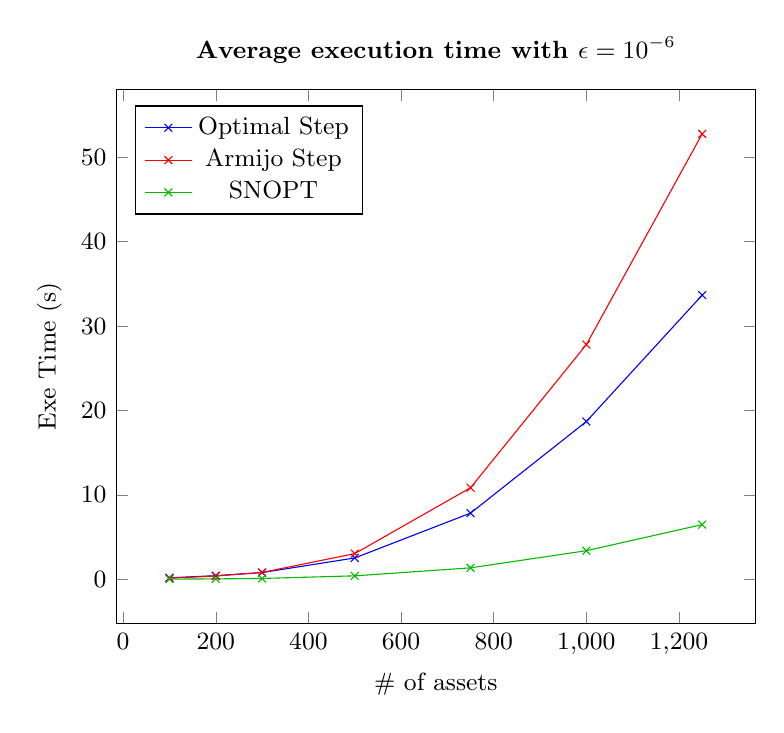
\begin{tikzpicture}
\begin{axis}[%
width=0.8\textwidth,
xlabel={\# of assets},
ylabel={Exe Time (s)},
legend pos=north west,
title=\textbf{Average execution time with {$\epsilon=10^{-6}$}},
]
\addplot [color=blue,solid,mark=x,mark options={solid}]
  table[row sep=crcr]{%
%5	8.3		\\
%10	13.8		\\
%20	25.9		\\
%30	42.5		\\
%50	.088		\\
%75	.141		\\
100	.167	\\
200	.420	\\
300	.787 	\\
500	2.519  	\\
750	7.834		\\
1000 18.686		\\
1250 33.661 \\
%1500 55.57 \\
%2000 197.34 \\
};
\label{Subplot:exe_e6_exact}

\addplot [color=red,solid,mark=x,mark options={solid}]
  table[row sep=crcr]{%
%5	5.5		\\
%10	10.2		\\
%20	19		\\
%30	29.5		\\
%50	.0617		\\
%75	.104		\\
100	.122	\\
200	.374		\\
300	.803		\\
500	3.032	\\
750	10.84		\\
1000	 27.801	\\
1250 52.762\\
};
\label{Subplot:exe_e6_armijo}

\addplot [color=gr,solid,mark=x,mark options={solid}]
  table[row sep=crcr]{%
%5	8.3		\\
%10	13.8		\\
%20	25.9		\\
%30	42.5		\\
%50	.009		\\
%75	.019	\\
100	.010		\\
200	.039		\\
300	.091	\\
500	.399	\\
750	1.347		\\
1000 3.380		\\
1250 	6.470	\\
%2000 32.865 \\
};
\label{Subplot:exe_e8_snopt}
\addlegendentry{Optimal Step}
\addlegendentry{Armijo Step}
\addlegendentry{SNOPT}
\end{axis}
\end{tikzpicture}
}

\makebox[\textwidth][c]{
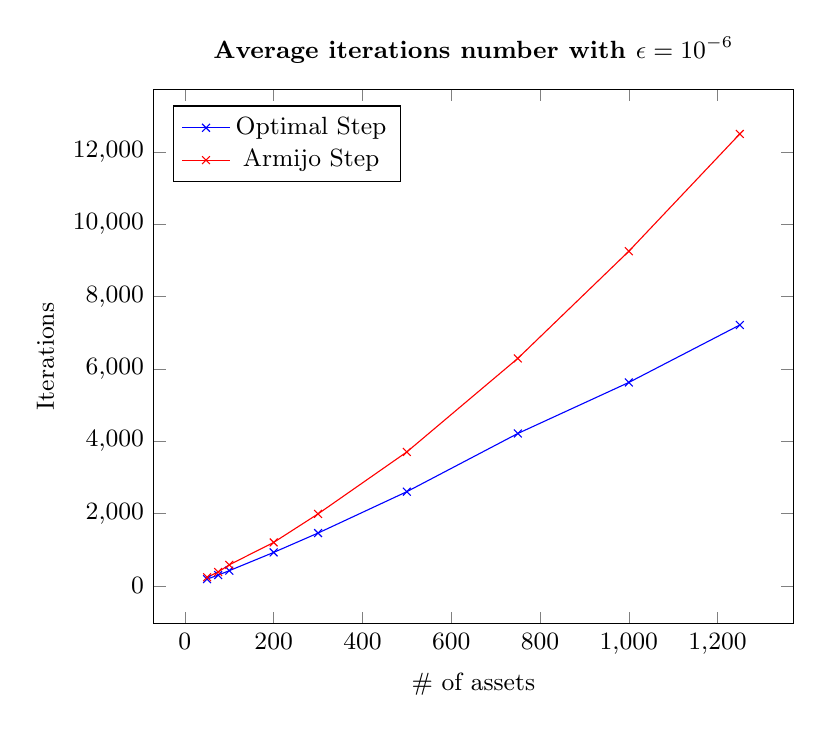
\begin{tikzpicture}
\begin{axis}[%
width=0.8\textwidth,
xlabel={\# of assets},
ylabel={Iterations},
scaled y ticks=false,
legend pos=north west,
title=\textbf{Average iterations number with {$\epsilon=10^{-6}$}}
]
\addplot [color=blue,solid,mark=x,mark options={solid}]
  table[row sep=crcr]{%
%5	22\\
%10	37\\
%20	68\\
%30	105\\
50	188\\
75	300\\
100	422\\
200	927\\
300	1462\\
500	2606\\
750	4215\\
1000	5626\\
1250	7215\\
};
\addplot [color=red,solid,mark=x,mark options={solid}]
  table[row sep=crcr]{%
%5	26		\\
%10	49		\\
%20	92		\\
%30	140		\\
50	240		\\
75	385		\\
100	584		\\
200	1203		\\
300	1992		\\
500	3705		\\
750	6292		\\
1000	9254	\\
1250	12498	\\
};
\addlegendentry{Optimal Step}
\addlegendentry{Armijo Step}
\end{axis}
\end{tikzpicture}
}
\end{figure}

\begin{figure}
\begin{tikzpicture}
\pgfplotsset{every tick label/.append style={font=\small}}
\pgfplotsset{every axis label/.append style={font=\small}}
\begin{axis}[
	ybar stacked,
	title=\textbf{Armijo line search},
    ylabel={\% Exe Time},
    xlabel={\# of assets},
    bar width = 18pt,
    width=0.8\textwidth,
    symbolic x coords={5, 10, 50, 100, 200, 300, 500, 1000},
    xtick=data,
    axis x line*=bottom,
    axis y line*=left,
    area legend,
    legend style={
    legend columns=5,
        at={(xticklabel cs:0.5)},
        anchor=north,
        draw=none
    }
    ]
\addplot[ybar, fill=step] plot coordinates {(5,52) (10,50) 
  (50,47) (100,42) (200,35) (300,27) (500,10) (1000,4)};
\addplot[ybar, fill=derivative] plot coordinates {(5,19) (10,19)(50,23) (100,29) (200,42) (300,57) (500,83) (1000,94)};
\addplot[ybar, fill=theta] plot coordinates {(5,12) (10,13) (50,13) (100,12) (200,10) (300,7) (500,2) (1000,1)};
\addplot[ybar, fill=violation] plot coordinates {(5,14) (10,13) (50,13) (100,13) (200,10) (300,8) (500,4) (1000,1)};
\addplot[ybar, fill=other] plot coordinates{(5,3) (10,5) (50,4) (100,4) (200,3) (300,1) (500,1)};
%\addlegendentry{Step}
%\addlegendentry{Gradient}
%\addlegendentry{Theta}
%\addlegendentry{Most Violating Pair}
%\addlegendentry{Others}
\end{axis}

\end{tikzpicture}

\begin{tikzpicture}
\pgfplotsset{every tick label/.append style={font=\small}}
\pgfplotsset{every axis label/.append style={font=\small}}
\begin{axis}[
    ybar stacked,
    title=\textbf{Optimal step computation},
    ylabel={\% Exe Time},
    xlabel={\# of assets},
    bar width = 18pt,
    width=0.8\textwidth,
    symbolic x coords={5, 10, 50, 100, 200, 300, 500, 1000},
    xtick=data,
    axis x line*=bottom,
    axis y line*=left,
    area legend,
    legend style={
    legend columns=5,
        at={(xticklabel cs:0.5)},
        anchor=north,
        draw=none
    }
    ]
\addplot[ybar, fill=step] plot coordinates {(5,73) (10,73) 
  (50,71) (100,67) (200,58) (300,48) (500,22) (1000,8)};
\addplot[ybar, fill=derivative] plot coordinates {(5,11) (10,10) (50,12) (100,17) (200,27) (300,40) (500,72) (1000,89)};
\addplot[ybar, fill=theta] plot coordinates {(5,7) (10,7) (50,7) (100,7) (200,6) (300,5) (500,2) (1000,1)};
\addplot[ybar, fill=violation] plot coordinates {(5,7) (10,7) (50,7) (100,7) (200,7) (300,6) (500,3) (1000,2)};
\addplot[ybar, fill=other] plot coordinates{(5,2) (10,3) (50,3) (100,2) (200,2) (300,1) (500,1)};
\addlegendentry{Step}
\addlegendentry{Gradient}
\addlegendentry{Theta}
\addlegendentry{Most Violating Pair}
\addlegendentry{Others}
\end{axis}
\end{tikzpicture}
\end{figure}

\clearpage
%% The Appendices part is started with the command \appendix;
%% appendix sections are then done as normal sections
%% \appendix

%% \section{}
%% \label{}

%% If you have bibdatabase file and want bibtex to generate the
%% bibitems, please use
%%
%%  \bibliographystyle{elsarticle-num} 
%%  \bibliography{<your bibdatabase>}

%% else use the following coding to input the bibitems directly in the
%% TeX file.

\begin{thebibliography}{00}
\section{Bibliography}
\bibitem{bai}
  	X. Bai, K. Scheinberg,
  	\emph{Alternating direction methods for non convex
  	optimization with applications to second-order
 	least-squares and risk parity portfolio selection},
  	2015.

\bibitem{snopt}
	P. E. Gill, W. Murray, M. A. Sanders,
	\emph{SNOPT: An SQP Algorithm for large-scale constrained optimization}, 
	2005.


\end{thebibliography}
\end{document}
\endinput
%%
%% End of file `elsarticle-template-num.tex'.
